\documentclass[runningheads,a4paper]{llncs}

\usepackage{amssymb}
\setcounter{tocdepth}{3}
\usepackage{subfigure}
\usepackage{graphicx}
\usepackage{url}
\urldef{\mailsa}\path|{cherish, yhhan}@koreatech.ac.kr|
\newcommand{\keywords}[1]{\par\addvspace\baselineskip
\noindent\keywordname\enspace\ignorespaces#1}

\begin{document}

\mainmatter  % start of an individual contribution

% first the title is needed
\title{SDN-based Distributed Mobility Management in LTE/EPC Network}

% a short form should be given in case it is too long for the running head
\titlerunning{SDN-based DMM in LTE/EPC Network}

% the name(s) of the author(s) follow(s) next
%
% NB: Chinese authors should write their first names(s) in front of
% their surnames. This ensures that the names appear correctly in
% the running heads and the author index.
%

\author{Yong-hwan Kim\inst{}
\and Youn-Hee Han\inst{}}
%
\authorrunning{Yong-hwan Kim et al.}
% (feature abused for this document to repeat the title also on left hand pages)

% the affiliations are given next; don't give your e-mail address
% unless you accept that it will be published
\institute{Advanced Technology Research Center \\ Korea University of Technology and Education, Korea \\
\email{\{cherish, yhhan\}@koreatech.ac.kr}}

%
% NB: a more complex sample for affiliations and the mapping to the
% corresponding authors can be found in the file "llncs.dem"
% (search for the string "\mainmatter" where a contribution starts).
% "llncs.dem" accompanies the document class "llncs.cls".
%

%\toctitle{Lecture Notes in Computer Science}
%\tocauthor{Authors' Instructions}
\maketitle


\begin{abstract}
As smart phone has rapidly proliferated over the past few years, mobile data traffic is expected to increase largely. Accordingly, LTE operators endeavor to cope with such increase in data volumes. The evolution of mobile network architectures toward flat architectures is being considered as a key solution to manage the explosion of mobile data traffic. To solve such problems, we propose a new SDN-based distributed mobility management supporting distributed P-GWs and virtually-centralized control plane. For enhancing network performance more, we also propose a route optimization strategy for internal traffic exchanged between LTE users. The proposed solutions' performance are compared with the conventional LTE/EPC network's scheme in terms of the P-GW data processing volume per unit time and the number of valid data sessions. The comparison results showed that the proposed solution can be an efficient way to enhance the scalability of LTE/EPC core network.

\keywords{Distributed Mobility Management, Dynamic Mobility, LTE/EPC, SDN}
\end{abstract}


\section{Introduction}
Due to the increasing popularity of smart-phones and other mobile devices, mobile data traffic is expected to continuously increase with an annual rate above $100\%$ \cite{ref1}, \cite{ref2}. Accordingly, LTE operators are in urgent need of means to cope with such increase in data volumes. The evolution of mobile network architectures toward flat architectures is being considered as a key solution to cope with the explosion of mobile data traffic \cite{ref3}-\cite{ref5}. For this, IETF Distributed Mobility Management (DMM) working group is trying to make standardizations of IP mobility anchors at an access network level \cite{ref6,ref7}. 

As 3GPP evolves to the Evolved Packet Core (EPC) network, the network hierarchy is also being flattened. In the hierarchy, the number of LTE/EPC network elements decreases, where the main elements in the data plane are Packet Data Network Gateway (P-GW), Serving Gateway (S-GW), and Evolved Node B (eNodeB). The number of hierarchy levels is reduced in the EPC network compared with the GPRS/UMTS network. In later deployment, P-GW and S-GW are expected to be co-located in the same physical element, thus the number of different network elements will be further reduced. In this hierarchy, P-GW provides access to Packet Data Network (PDN) by assigning an IP address to User Equipments (UEs) and serves as the mobility anchor point. UEs do not change their mobility anchor points if they remain attached to the same operator's access network. So, all data traffic for an UE is routed over P-GW and thus P-GW is needed to handle it.

As another trends in mobile networks, Software-Defined Networking (SDN) and Network Functions Virtualization (NFV) are being actively adopted by mobile operators. SDN and NFV can enable resource and service orchestration with dynamic provisioning by deploying and utilizing virtually-centralized control plane. In parallel with DMM technology, SDN and NFV will lead to the deployment of more flatter systems in which mobility anchor points can be placed closer to the UEs and the local breakout/traffic offload can be facilitated \cite{ref8}. Furthermore, a virtually centralized control plane allows for more flexibility by having the S-/P-GWs data-plane deployed in a distributed manner \cite{ref8-1}. It is however expected that the change of UE's mobility anchors upon handover will happen far more often due to high number of mobility anchors deployed at access networks. So, DMM should efficiently keep ongoing sessions active in case of handovers that require mobility anchor change. 

In this paper, we propose a new distributed LTE/EPC network architecture based on SDN and NFV supporting distributed P-GWs. It is designed based on the following requirements: 1) Distributing P-GWs closer to the UEs, 2) Virtually centralizing control plane, 3) Separation of the control and data planes, and 4) Efficient mobility management. We also propose the route optimization for internal traffic exchanged by LTE/EPC UEs to enhance network performance. We have implemented the proposed solution on NS3-LENA simulation environment, \cite{ref13,ref13-1}. The proposed solution's performance is compared with the conventional LTE/EPC network system's scheme in terms of the P-GW data processing volume and the number of valid data sessions. The comparison results show that the proposed LTE/EPC architecture and DMM solution can be a more efficient way to support the scalability of LTE/EPC core network.

The rest of this paper is organized as follows. Section 2 proposes a SDN-based DMM approach in LTE/EPC. Section 3 investigates the performance of our proposal by simulations, and Section 4 finally concludes this paper.

\begin{figure}[t]
\begin{center}
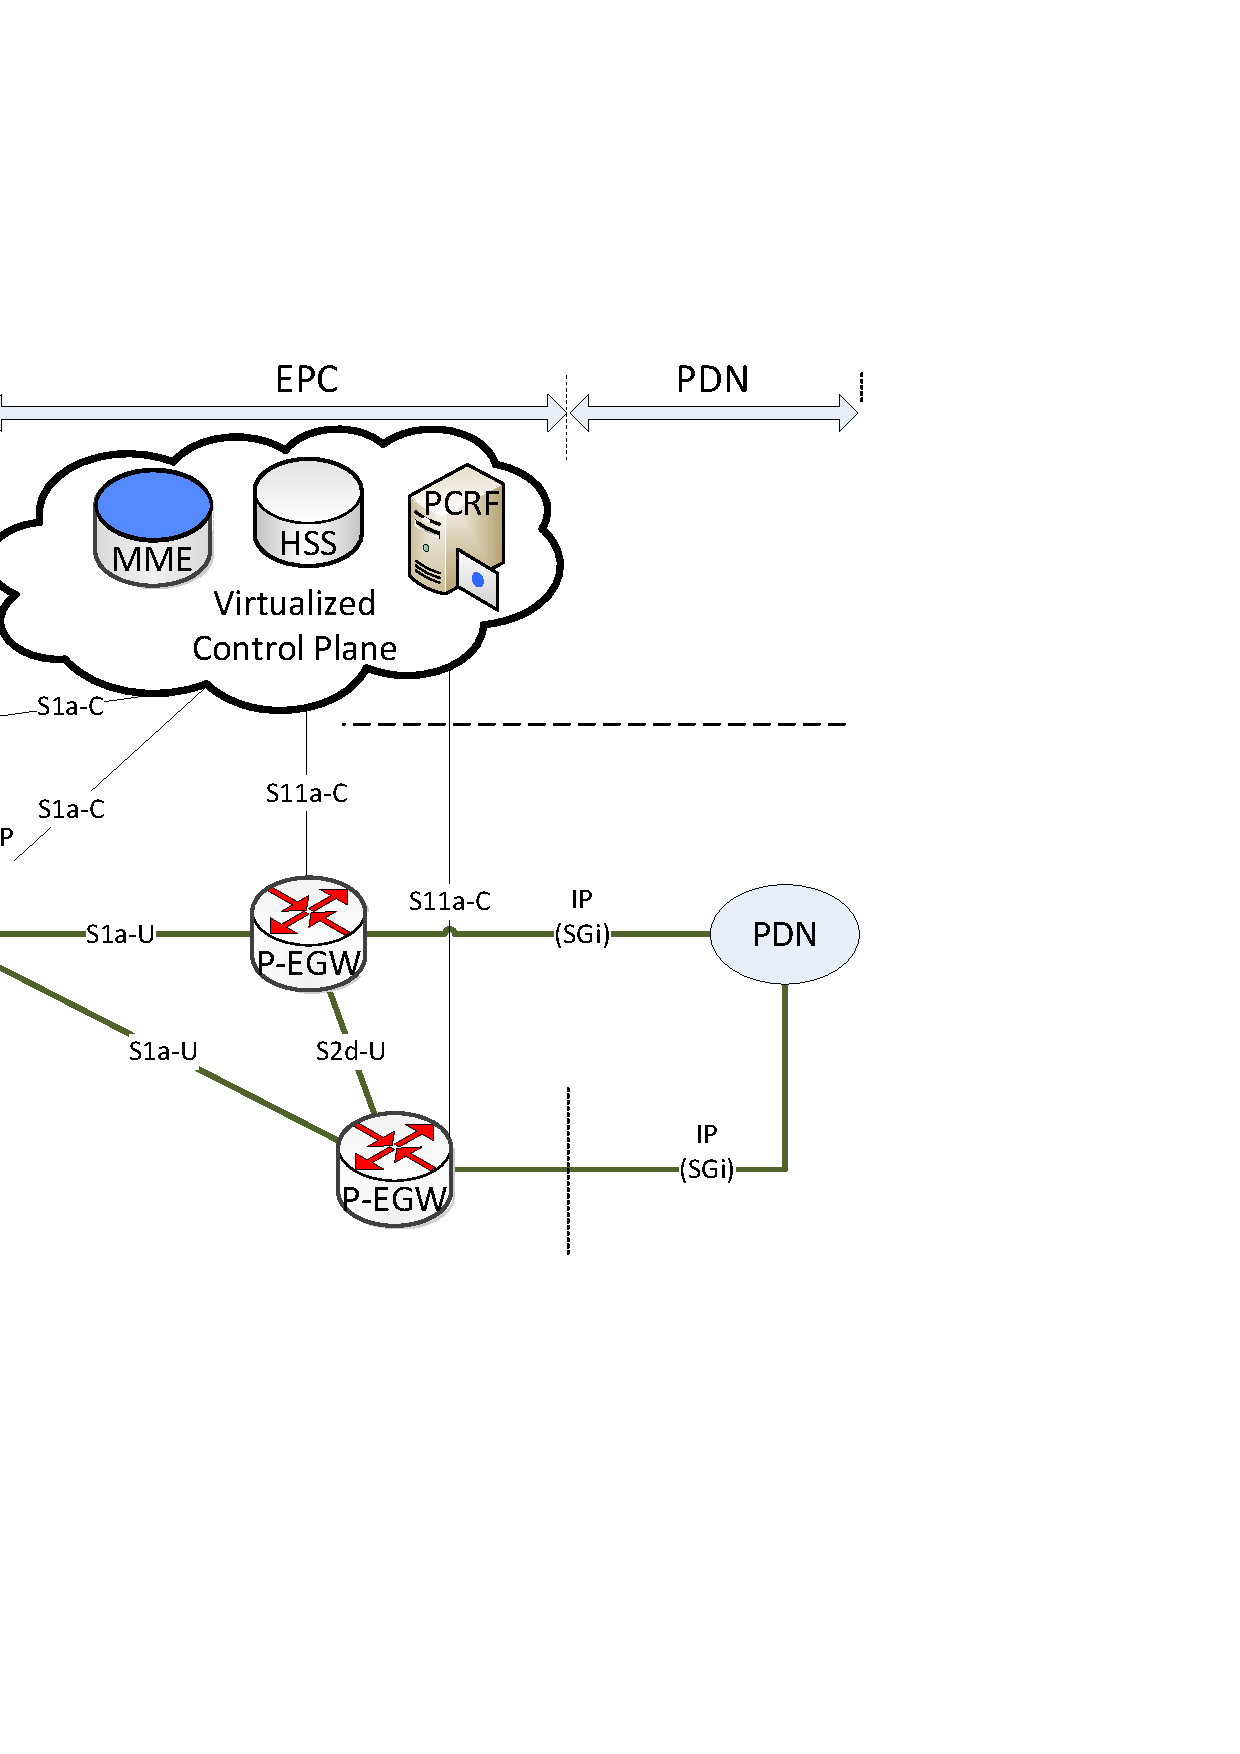
\includegraphics[width=9cm]{figures/fig1.pdf}
\end{center}
\caption{Reference model for a SDN-based DMM architecture in LTE/EPC.}
\label{fig:f1}
\end{figure}


\section{Proposed SDN-based DMM approach}
\subsection{Proposed SDN-based DMM architecture}
Fig.\ref{fig:f1} shows the reference model for our SDN-based DMM (SDMM) architecture in LTE/EPC. It is designed as three requirements about how to redesign LTE/EPC network:

    1) \textit{Distributing data plane:} Instead of employing a single centralized infrastructure based on P-GW, multiple distributed components can be deployed in different areas of the network. A new network element, named packet data network edge gateway (P-EGW), is so similar to the existing P-GW in term of the functionalities and the roles. However, P-EGWs will be deployed near to the radio area network (RAN), so that their location will be somewhere between eNB and S-GW. P-EGW has also the role as SDN switch to communicate with SDN controller in a virtually and centralized control plane. The distributing data plane allows scalability and flexibility to network;

    2) \textit{Virtually centralizing control plane:} The virtually control plane is consists of MME, HSS, and PCRF being in charge of control parts in conventional LTE/EPC network. It is a cloud form using NFV and can communicate with the entities in data plane via SDN technology. The centralizing control plane can provide flexible and dynamic framework for optimization to network;

    3) \textit{Separation of the control and data planes:} In order to totally separate the LTE/EPC network¡¯s data and control planes, SDN is adapted to not only EPC networks but also the edge of the network. In other words, the functions of whole network¡¯s entities including eNodeB, distributed P-GW, MME, and the others should be separated into the data and control planes and then should be managed by SDN technology. The separation of the control and data planes allows sophisticated traffic management to be driven by software, rather than purely by hardware routers.

\begin{figure}[t] 
\centering 
\subfigure[Movement from P-EGW $\#1$ to P-GEW $\#2$]{
	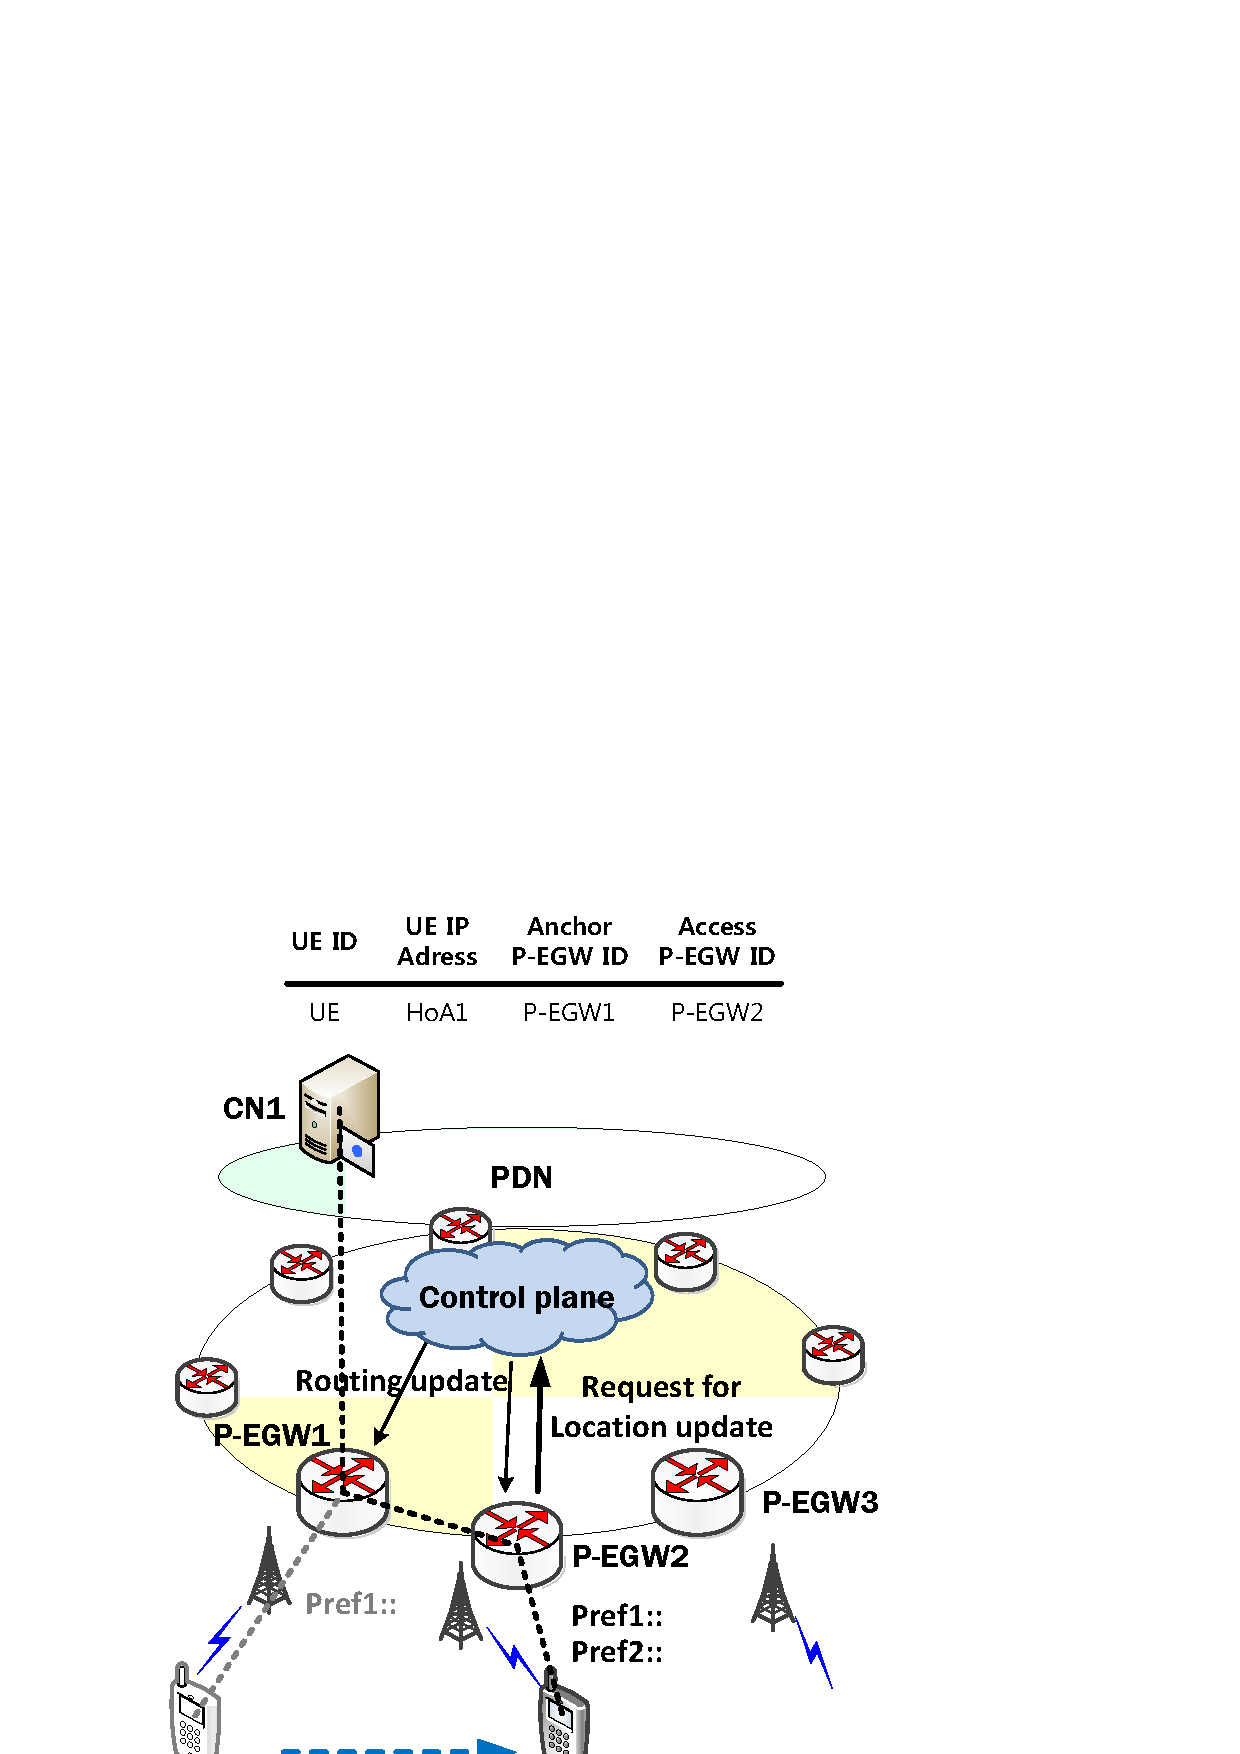
\includegraphics[width=0.45\linewidth, trim=0cm 0cm 0cm 0cm]{./figures/fig2(a).pdf}}
\subfigure[Movement from P-EGW $\#2$ to P-GEW $\#3$]{
	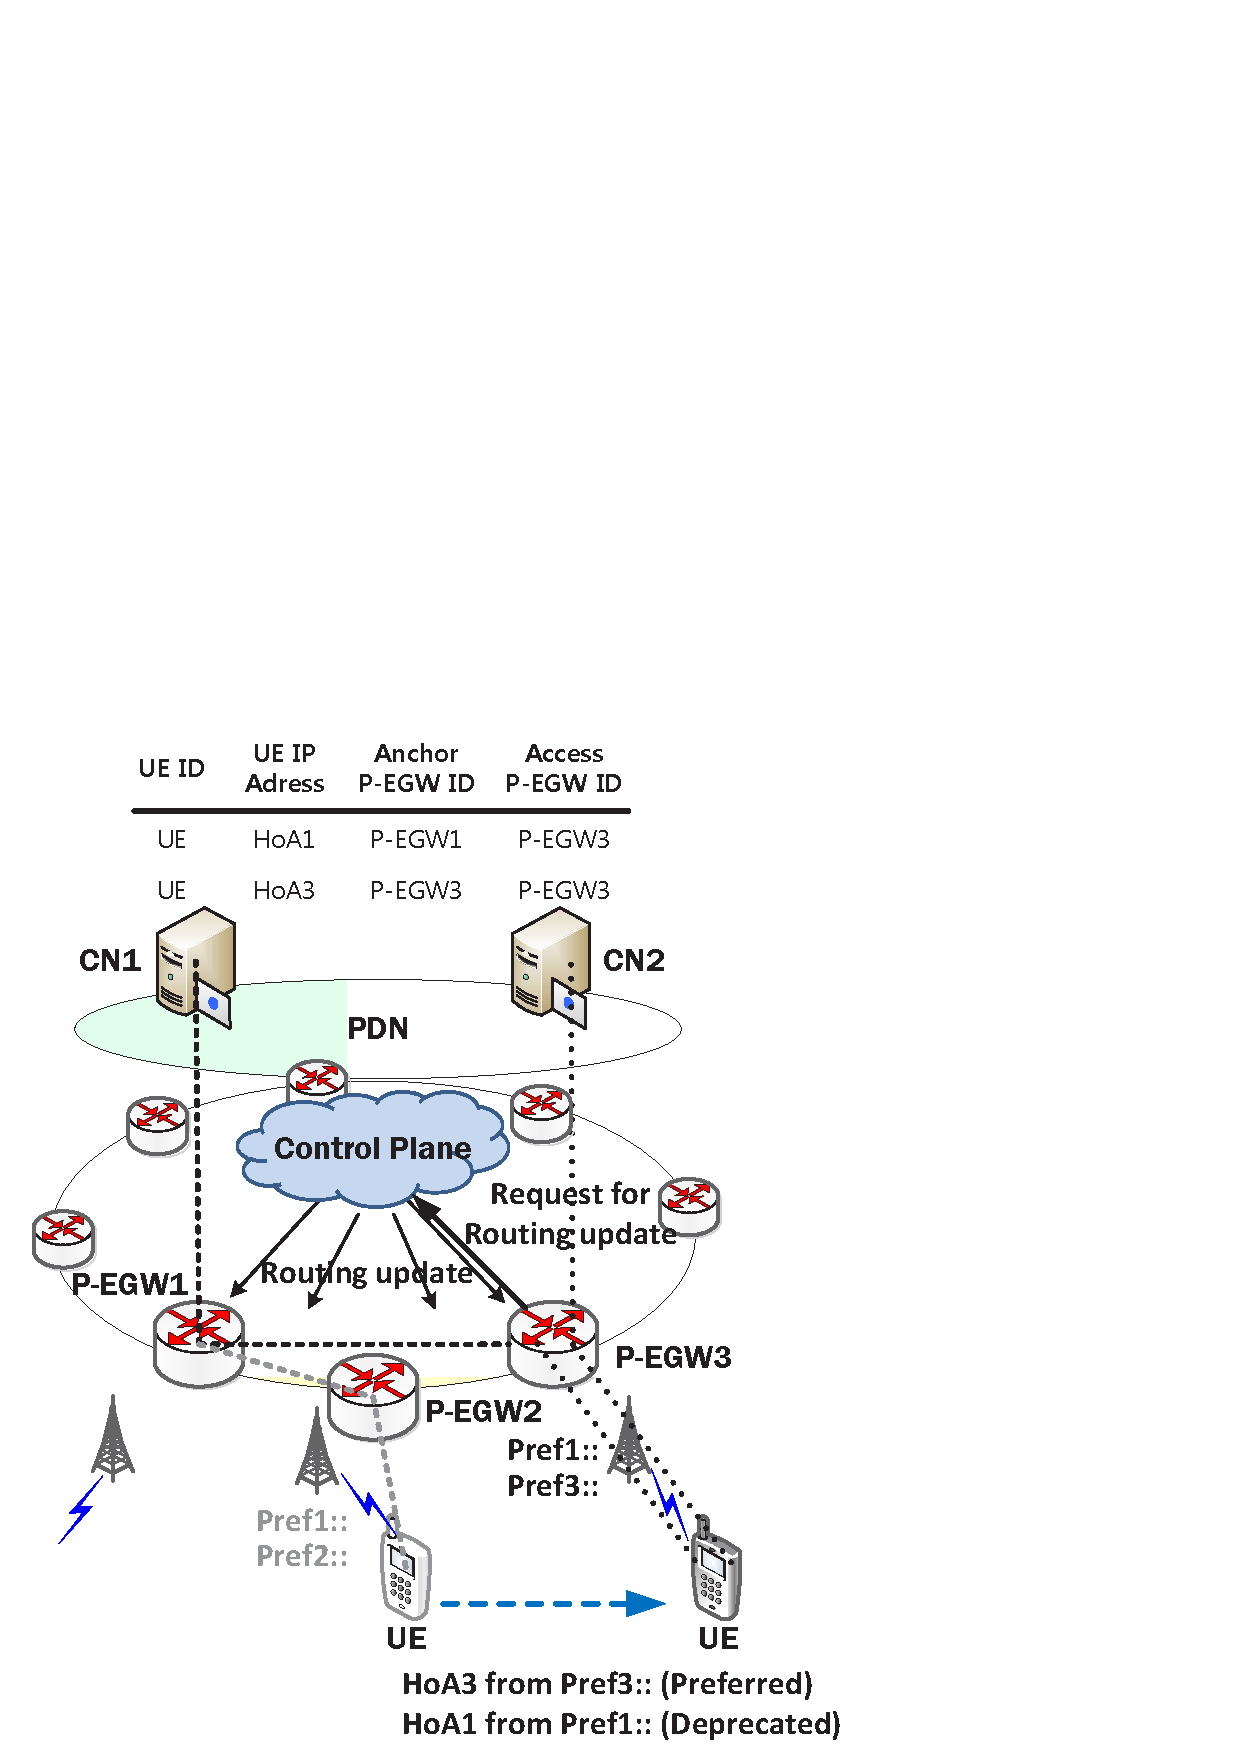
\includegraphics[width=0.45\linewidth, trim=0cm 0cm 0cm 0cm]{./figures/fig2(b).pdf}}
\caption{Examples for proposed SDMM}
\label{fig:2}
\end{figure}

\subsection{Proposed SDN-based DMM}

The proposed SDMM makes use of a routing protocol to support UE's mobility, instead of a tunnel protocol. The routing protocol is running in the control plane centralized cloud form. The routing update message between the control plane and P-EGW having role of SDN switch will be exchanged via SDN technology. It can provide a selective routing update method.

When the MN initially attaches to an anchor P-EGW, it obtains an IP address called HoA. HoA is then internally advertised within the domain using an intra-domain protocol (e.g., IBGP). When the UE moves and attaches to a different P-EGW (Access P-EGW), the access P-EGW finds out the address assigned to the UE during the authentication phase via SDN controller in the control plane. And then, a routing update between the anchor P-EGW and the access P-EGW is performed for session continuity by SDN controller in the control plane. In this way, the reachability of the UE is ensured while moving within the LTE/EPC network.

Meanwhile, when the UE in a new P-EGW's area tries to create a new PDN connection, the new P-EGW is in charge of creating the new PDN connection as the Anchor P-EGW. That is, a UE can have multiple PDN connections through multiple anchor P-EGWs. Therefore, these IP addresses related with multiple P-EGW will be managed simultaneously. For this, the SDMM adopts distributed logical interface (DLIF) presented in \cite{ref10}.

A location information of UE in the proposed LTE/EPC network is <UE ID, UE IP Address, Anchor P-EGW ID, Access P-EGW ID> per UE's PDN connection. UE IP Address is unique for PDN connection anchored P-EGW. Anchor P-EGW ID and Access P-EGW ID are needed for finding the location of UE in distributed data plane. This location information of UE is naturally managed by this control plane. However, if the network system uses the other factor for data routing and forwarding and this factor is assigned per P-EGW, another factor can be used instead of UE IP Address.

An example of this solution is shown in Fig. \ref{fig:2}. In Fig. \ref{fig:2}(a), a UE initially attaches to P-EGW $\#1$ as anchor P-EGW and communicate with CN $\#1$ in PDN. And then the UE move to P-EGW $\#2$, P-EGW $\#2$ acquires UE's information including address during the authentication phase via SDN controller in the control plane. And then P-EGW $\#2$ request for routing update to the control plane via SDN. If the control plane receives this request, the control plane will perform a routing update between P-EGW $\#1$ and access P-EGW $\#2$. When the routing update is finished, the session data anchored P-EGW $\#1$ between the UE and CN $\#1$ is redirected to P-EGW $\#2$. In \ref{fig:2} (b), the UE move to P-EGW $\#3$, the session data anchored P-EGW $\#1$ between the UE and CN $\#1$ is redirected to P-EGW $\#3$ though the same procedures. Meanwhile, when the UE create a new session to CN $\#2$ in PDN, P-EGW $\#3$ is anchor P-EGW for new session using new IP address. In this procedure, P-EGW $\#3$ can create DLIF related with P-EGW $\#1$, and then P-EGW $\#3$ can send not only P-EGW $\#3$'s RA message but also P-EGW $\#1$'s RA message. At that time, P-EGW $\#3$ do not have to create DLIF related with P-EGW $\#2$ because there is no the session anchored P-EGW $\#2$.

The data transfer after the movement of a UE in the SDMM is handled by suboptimal path not optimal path. However, this approach can reduce amount of signal messages related with routing update and the handover latency compared with previous routing based DMM approaches \cite{ref11}, \cite{ref12}. However, the introduction of DLIF can solve this problem to some degree. Furthermore, it can be remove the cost related with tunnel compared with host and network based DMM approaches.

The assigned IP addresses of the UEs for a PDN connection managed the same network operator can be made up based on pre-defined prefix information related with P-EGW. Therefore, if the IP address has those pre-defined prefix, the data communication can be judged to be inner traffic between UEs in the network. In this case, the route for this data communication can be optimized by routing update between the P-EGWs for UEs by the SDN technology.


\section{Performance Evaluation}

In this section, we analyze the SDMM's performance compared to the one in the conventional LTE/SAE network in terms of the P-GW/PEGW¡¯s data processing volume per unit time and the number of valid data sessions. For the analysis, we used the open source simulator NS-3.16 \cite{ref13}, with the LENA LTE module (M4 release).

The simulation area is $30 km \times 30 km$. the one P-GW, four S-GWs, and thirty-six eNBs are inter-connected in the conventional LTE/SAE network. On the other hand, twelve P-EGWs instead of P-GW and S-GWs in SDMM are deployed. They are directly connected to just three eNBs. Each wired link is a full-duplex link and provides a bandwidth of $10 Gbps$. The delay of each link was configured to be the one between $25 ms$ and $125 ms$ considering the distance among each node. The LTE wireless channel and modulation/encoding models are set to be the default models provided by NS-3.16-LENA. In the experiment, we deployed $100$ UEs randomly in the area and traffic model is a voice over IP traffic. So, UE having even IMSI sends 80 Bytes UDP data to UE having odd IMSI every 10ms (64Kbps)

\begin{figure}[t] 
\centering 
\subfigure[Data throughput]{
	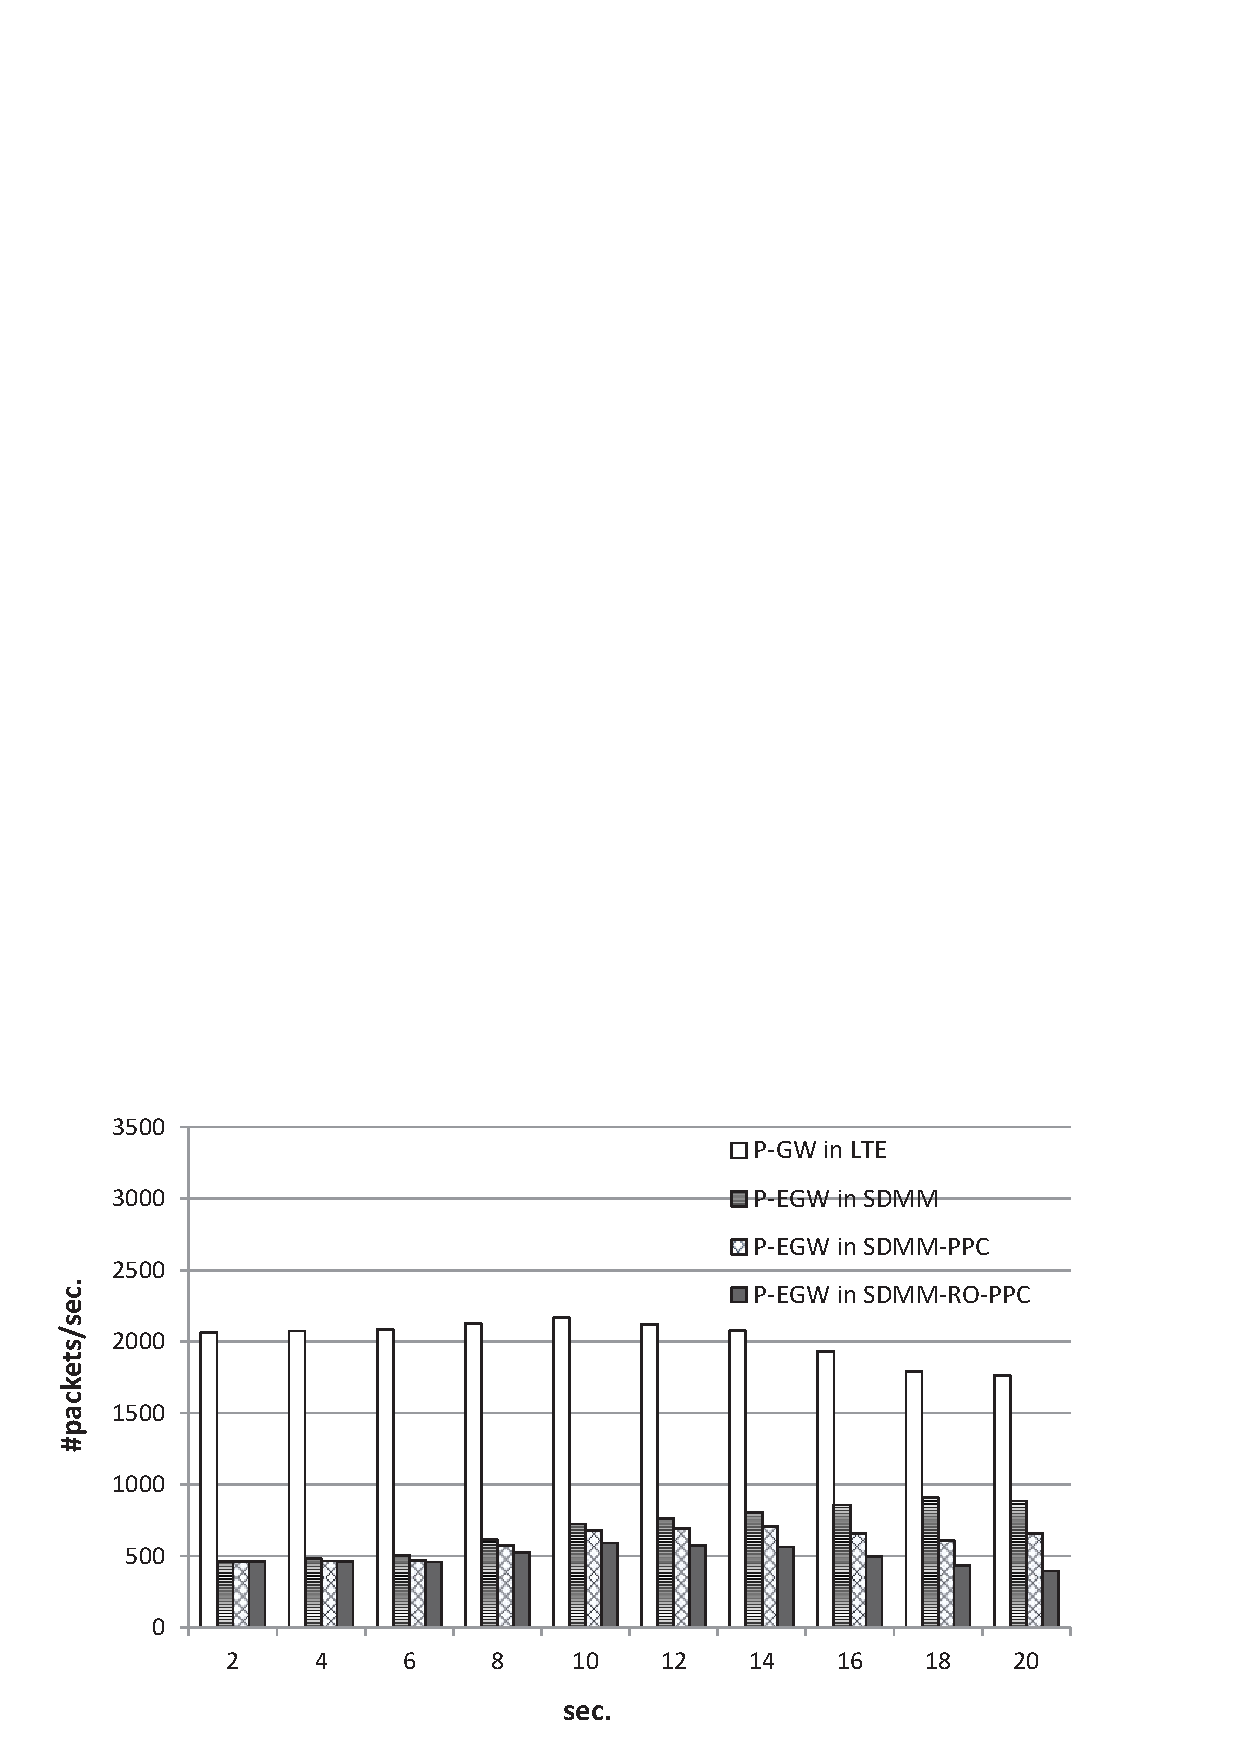
\includegraphics[width=0.45\linewidth, trim=0cm 0cm 0cm 0cm]{./figures/fig3.pdf}}
\subfigure[The number of valid data sessions]{
	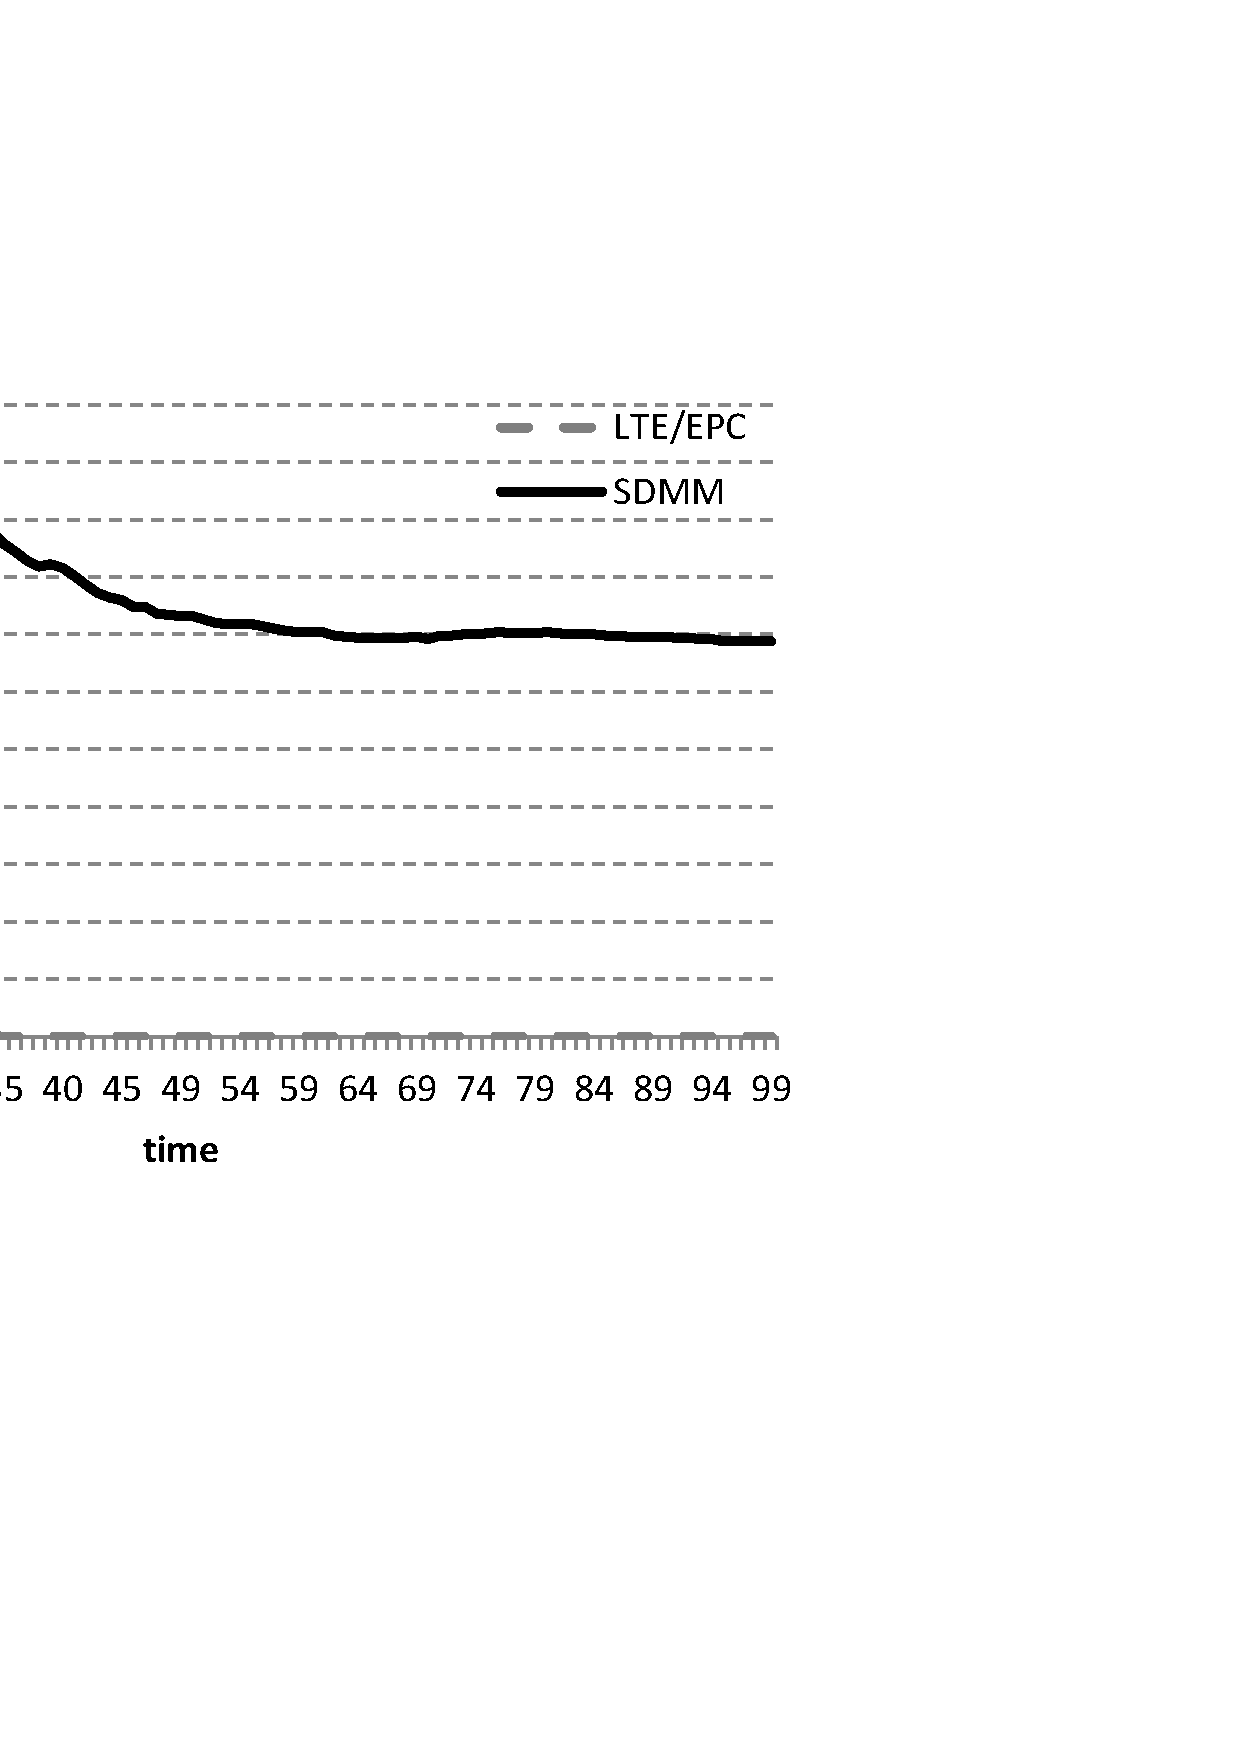
\includegraphics[width=0.45\linewidth, trim=0cm 0cm 0cm 0cm]{./figures/fig4.pdf}}
\caption{Simulation results between SDMM and conventional LTE}
\label{fig:2}
\end{figure}

Fig. \ref{fig:3} (a) shows the P-GW and the P-EGW¡¯s data processing volume per unit time in traffic scenario. In the figure, the data processing volume of P-EGWs in all cases (SDMM, SDMM-PPC(Dynamic mobility management), SDMM-RO-PPC) is quite less than that of P-GW in the beginning of simulation due to the distributed architecture of P-EGWs. On the other hand, the total amount of data processing volume across all P-EGWs is more than the data processing volume of P-GW. It is due to the data traffic caused by routing between P-EGWs. However, as time goes by, the data processing volume of P-EGWs increases in the order of SDMM $\>$ SDMM-PPC $\>$ SDMM-RO-PPC. Especially, the one of the SDMM-RO-PPC is not nearly affected by the passing time.

Fig. \ref{fig:3} (b) plots the number of valid sessions in the conventional and proposed LTE/EPC networks. A session is valid in terms of service quality if its packet drop rate iFs lower than 10$\%$. In the experiment, we deployed $100$ UEs randomly in the area and configured each UE to create a new session composed of 1Mbps UDP data traffic with another UE every 40ms. A handover situation was not generated. As shown in the figure, the SDMM (SDMM$\#1$, SDMM$\#2$) can create valid sessions twice more than the conventional LTE/EPC network (LTE). Data traffic are concentrated to the P-GW in the conventional LTE/EPC network, while there is not such a single point in the SDMM and all data traffic are directly tunneled between P-EGWs. That is, the SDMM does not suffer from the bottleneck problem at a specific node in the network, and thus it is more scalable than one of the conventional LTE/EPC network. In addition to that, SDMM can permit more the number of UE and the data traffic volume as the number of deployed P-EGW is more larger and the PEGWs is deployed close to the RAN.


\section{Conclusions}


In this thesis, a new distributed LTE/EPC network architecture based on SDN and NFV supporting P-EGWs is proposed. In addition, the distributed mobility management, called SDMM, which is proper to the proposed architecture, is also proposed. For the performance evaluation, the proposed solution is implemented on the NS-3 LENA. The performance of the proposed solution was compared with the conventional LTE/EPC network system in terms of the P-GW/PEGW's data processing volume per unit time and the number of valid data sessions. The comparison results showed that the proposed LTE/EPC architecture and their DMM solution can be a more efficient way to support the scalability of LTE/EPC core network.
.
The proposed solution will give LTE network operator increased scalability, flexibility, cost savings in short-term. Furthermore, this solution concept will allow for new service architectures, service exposure, new revenue opportunities and more efficient operations in the long term.

%\subsubsection*{Acknowledgments.} This research was supported by Basic Science Research Program through the National Research Foundation of Korea (NRF) funded by the Ministry of Education (2013R1A1A2010050), and also financially supported by the Ministry of Knowledge Economy (MKE) and Korea Institute for Advancement of Technology (KIAT) through the Workforce Development Program in Strategic Technology.

\begin{thebibliography}{4}

\bibitem{ref1} Morgan Stanley Reports, "Internet Trends," Apr. 2010.

\bibitem{ref2} "Cisco Visual Networking Index: Global Mobile Data Traffic Forecast Update, " Cisco White Paper, 2011-2016, Feb. 2010.

\bibitem{ref3} P. Bertin, S. Bonjour, and J.-M. Bonnin, "A Distributed Dynamic Mobility Management Scheme designed for Flat IP Architectures," In Proc. of International Conference on New Technologies, Mobility and Security (NTMS), Nov. 2008.

\bibitem{ref4} P. Bertin, S. Bonjour, and J.-M. Bonnin, "Distributed or Centralized Mobility?, " In Proc. of IEEE Global Communications Conference (GLOBECOM), Dec. 2009.

\bibitem{ref5} H A. Chan, H. Yokota, J. Xie, P. Seite, D. Liu, "Distributed and Dynamic Mobility Management in Mobile Internet: Current Approaches and Issues," Journal of Communications, Vol 6, No 1 (2011), 4-15, Feb. 2011

\bibitem{ref6} H. Chan, et al., "Requirement of Distributed Mobility Management," IETF Internet Draft, draft-chan-dm mrequirements-00, March 2012.

\bibitem{ref7} B. Sarikaya, "Distributed Mobile IPv6," IETF Internet Draft, draftsarikaya-dmm-dmipv6-00, Feb 2012.

\bibitem{ref8} Y. Wang and J. Bi, "A solution for IP mobility support in software defined networks," In Proc. of 23rd ICCCN, 2014.

\bibitem{ref8-1} L. Valtulina, M. Karimzadeh, G. Karagiannis, G. Heijenk, and A. Pras, "Performance Evaluation of a SDN/OpenFlow-Based Distributed Mobility Management (DMM) Approach in Virtualized LTE Systems," In Proc of Globecom 2014 Workshop - Cloud Computing Systems, Networks, and Applications, 2014.

\bibitem{ref9} P. Seite and P. Bertin, "Distributed Mobility Anchoring," IETF Internet Draft, draft-seitedmm-dma-00, Feb. 2012.

\bibitem{ref10} T. Melia et al., ¡°Logical Interface Support for multi-mode IP Hosts,¡± IETF Internet draft, draft-ietf-netext-logical-interface-support-10 (work in progress), Sep. 2014

\bibitem{ref11} P. McCann, "Authentication and Mobility Management in A Flat Architecture," IETF Internet-Draft, draft-mccann-dmm-flatarch-00 (work in progress), Mar. 2012.

\bibitem{ref12} H. Chan and K. Pentikousis, "Enhanced Mobility Anchoring," IETF Internet draft, draft-chan-dmm-enhanced-mobility-anchoring-00 (work in progress), Jul. 2014.

\bibitem{ref13} NS3 network simulator. http://www.nsnam.org/

\bibitem{ref13-1} LENA Design Documentation. http://lena.cttc.es/manual/lte-design.htm

\end{thebibliography}

\end{document}
